This chapter provides detailed specifications of the system under development.

\section{Functional Requirements}

% This section describes each function/feature provided by our system. These functions are logically grouped into modules based on their purpose/users/mode of operations etc (as per our system). A functional hierarchy may look like:
Functional requirements are grouped into modules corresponding to major system components. 
\begin{outline}
  \1 Core Chatbot Module (Public Facing)
  \2 Multimodal Input Handling
  \3 Text Input: Accept text queries in English, Urdu, and Roman Urdu (basic level).
  \3 Image Input: Analyze uploaded images for contextual information (e.g., payment receipts, prescriptions, donation screenshots). Handwritten text recognition is out of scope for MVP. 
  \3 Voice Input (Phase 2 - Conditional): Convert voice messages to text using Speech-to-Text API. Basic Urdu support only; dialect variations are out of scope. Voice integration depends on successful testing of Phase 1 text-based system. 
  \4 \textit{MVP Scope: Phase 1 focuses on duo-lingual text (English + Urdu) and image input only.}
  \2 Intent Classification \& Domain Identification 
  \3 Domain Classification: Automatically identify the query domain from four categories:  
  \4 Donation: Payment methods, project details, Zakat/Sadaqah eligibility 
  \4 Healthcare: Hospital locations, services, appointments, ambulances 
  \4 Blood Services: Donor eligibility, blood bank locations, blood group availability 
  \4 General Inquiry: Organization information, volunteering, events, queries about other domains
  \4 \textit{Note: this does not cover the exhaustive list of data for the domains mentioned}
  \3 Intent Clarification Loop: When queries are ambiguous or confidence score is low, prompt user with clarifying questions before proceeding (e.g., "Are you asking about blood donation or healthcare services?"). 
  \3 Confidence Threshold: Queries with confidence score below 0.7 are flagged for human escalation. 
  \2 Contextual Response Generation 
  \3 RAG-Based Retrieval: Retrieve verified information from the domain-structured knowledge base using Retrieval-Augmented Generation. 
  \3 Persona-Aware Responses: Adapt response length, tone, and detail based on identified user persona (e.g., overseas donor, non-tech-savvy patient, recurring donor). 
  \3 Follow-Up Context: Maintain session context to handle follow-up questions that depend on prior conversation history. 
  \3 Session Management: Preserve conversation context throughout the user session to enable multi-turn dialogues.
  \2 Multilingual Response \& Accessibility 
  \3 Language Selection: Allow users to select their preferred language (English or Urdu) at the start of interaction. 
  \3 Quick Reply Options: Provide button-based shortcuts and pre-defined options for low-literacy users to minimize typing. 
  \3 Consistent Quality: Ensure response quality is consistent across languages with no discrepancy between English and Urdu outputs. 
  \2 Trust \& Verification
  \3 Branding Display: Show verified Alkhidmat branding, official logos, and chatbot verification messages to assure users of authenticity. 
  \3 Official Channel Verification: Display verified WhatsApp Business number and official website domain to prevent scam concerns. 
  \2 Guardrails \& Safety 
  \3 Content Moderation: Implement guardrails to prevent inappropriate responses or off-topic conversations. 
  \3 Privacy Protection: Ensure no personal data is retained beyond the session lifetime. 
  \3 Fallback Responses: Provide predefined safe responses when the system cannot confidently answer a query. 
  
  \1 Information Retrieval \& Data Management Module \\
  The knowledge base contains periodically updated, domain-structured information covering (note: this is not an exhaustive list of the data for each domain): 
  \2 RAG Knowledge Base (General Information) 
  \\\textit{Note: Knowledge base is NOT real-time; it is periodically updated by administrators. }
  \3 Donation Support: 
  \4 Active and verified campaign details (healthcare, education, orphan care, women empowerment, disaster relief) 
  \4 Payment methods and step-by-step guidance (Easypaisa, JazzCash, bank transfer, international cards, PayPal)
  \4 Zakat and Sadaqah eligibility criteria for different programs 
  \4 Donation workflow and confirmation processes
  \4 Transparency reports and impact summaries 
  \3 Healthcare Information: 
  \4 List of Alkhidmat hospitals, clinics, labs, and pharmacies with addresses and coordinates 
  \4 Service offerings per facility (OPD, diagnostics, pharmacy, ambulance) 
  \4 Operating hours and appointment procedures
  \4 Consultation fees, test charges, and medicine pricing
  \4 Doctor availability, specializations, and gender-specific staff information 
  \4 Emergency helpline numbers and ambulance booking procedures 
  \3 Program Information: 
  \4 Summaries of Alkhidmat's 12+ domains (education, water, orphan care, community services, disaster management)
  \4 Women-centric initiatives (Bano Qabil, maternity services, women empowerment) 
  \4 Youth and student programs 
  \4 Corporate Social Responsibility (CSR) partnership opportunities 
  \3 General Information: 
  \4 Organization history, mission, and credibility verification 
  \4 Volunteering opportunities and community event schedules
  \4 FAQs on trust, transparency, and fund utilization 
  \2 Blood Donation Microservice (Operational Data) \\
  A separate microservice containing transactional and inventory information integrates with the main system to handle blood donation queries: 
  \3 Donor Eligibility Validation: Check eligibility based on age, weight, hemoglobin levels, blood pressure, and donation intervals (WHO and Alkhidmat internal SOPs).
  \3 Blood Bank Locations: Retrieve nearest Alkhidmat-licensed blood bank addresses and contact information based on user location. 
  \3 Blood Group Availability: Query current blood stock levels and urgent blood group requirements. 
  \3 Donation Process Information: Provide step-by-step donation process details (registration, screening, donation, post-care instructions). 
  \3 Donor Network Registration: Allow users to register for SMS/WhatsApp alerts when their blood group is urgently needed. 
  \3 Post-Donation Guidelines: Provide medical instructions (hydration, rest, when to resume activities). 
  \3 Recipient Support: Guide blood recipients on required documents (CNIC, prescription), cross-match duration, reservation policies, and service charges. 
  \2 User Profiling \& Persona Management (Contextual Database) \\
  Maintain a separate database to store user information and enable personalized interactions: 
  \3 Persona Classification: Classify users into personas based on interaction patterns using a donor-beneficiary matrix:  
  \4 Donor personas: Overseas, Local, Recurring, First-Time, Corporate, Non-tech Savvy 
  \4 Healthcare personas: Rural/Urban Patient, New Patient, Non-tech Savvy Patient 
  \4 Blood service personas: New/Recurring Blood Donor, Blood Recipient 
  \3 Interaction History Tracking: Record user query patterns, preferred language, interaction frequency, and topics of interest. 
  \3 Dynamic Persona Updates: Update user persona classification after each interaction based on new behavioural data. 
  \3 Context-Aware Response Adaptation: Tailor response length, explanation depth, and recommendations based on identified persona (e.g., provide detailed explanations for first-time donors, concise responses for recurring donors).
  \3 Personalized Recommendations: Suggest relevant campaigns, services, or programs based on user history and persona. 
 
  \1 Human Agent Dashboard (Staff Facing) 
  \2 Escalation \& Routing 
  \3 Automatic Escalation: Forward queries with confidence score below 0.7 to relevant department-based chat agents.
  \3 Domain-Based Routing: Route escalated queries to specialized agents (Donation team, Healthcare team, Blood Services team, General Support). 
  \3 Sensitive Query Handling: Automatically escalate queries involving complaints, refunds, or personal grievances to human agents. 
  \2 Conversation Management
  \3 Real-Time Takeover: Allow human agents to join ongoing conversations within the same chat thread without disrupting user experience. 
  \3 24-Hour WhatsApp Window: Enable agents to respond within the 24-hour WhatsApp Business API interaction window.
  \3 Pre-Approved Templates: Provide agents with Meta-approved message templates for initiating conversations outside the 24-hour window. 
  \3 Conversation History Access: Enable agents to view full conversation context before responding. 
  \2 Knowledge Base \& Dialogue Management
  \3 Content Updates: Allow administrators to add, modify, or archive FAQs and program information in the RAG knowledge base. 
  \3 Dialogue Flow Definition: Enable admins to define and update pre-approved greeting messages, fallback responses, and guided conversation flows. 
  \3 Guardrail Configuration: Provide admin interface to set and adjust content moderation rules and response boundaries.
  \2 Role-Based Access Control 
  \3 Chat Agent Access: Grant domain-specific agents access only to queries within their department. 
  \3 Admin Privileges: Provide full system access to administrators for knowledge base management, guardrail settings, and user management. 
  \3 Audit Trail: Log all agent actions (view, respond, resolve) with timestamps for accountability. 

  \1 Analytics \& Logging Module 
  \2 Usage Tracking 
  \3 Query Metrics: Record total queries, query volume by domain, peak usage times, and average session duration. 
  \3 Response Time Monitoring: Track response time per query (target: 3-15 seconds based on complexity). 
  \3 Escalation Rate Tracking: Monitor percentage of queries escalated to human agents by domain. 
  \2 User Feedback Collection 
  \3 Post-Interaction Rating: Prompt users for thumbs-up/thumbs-down rating 15-20 minutes after their last query.
  \3 Follow-Up Query Check: Send a message asking if the user has any remaining questions before requesting feedback. 
  \3 Satisfaction Score Calculation: Aggregate user satisfaction metrics over time. 
  \2 Performance Analysis 
  \3 Answer Accuracy Monitoring: Track percentage of queries resolved by AI without escalation (target: $\geq$90\%). 
  \3 Domain Performance: Analyze which domains have highest accuracy, longest response times, or most escalations. 
  \3 Trend Identification: Highlight common query topics and identify emerging information needs that require knowledge base updates. 
  \2 Reporting \& Insights
  \3 Dashboard Visualization: Provide real-time analytics dashboard for administrators showing KPIs and trends.
  \3 Export Functionality: Generate CSV/PDF reports of usage metrics for management review. 
  \3 Anomaly Detection: Flag unusual query patterns (e.g., spam, repeated failures, sudden traffic spikes). 

  \1 Out of Scope 
  \2 Handling of regional Urdu dialects is beyond the current scope. The system is designed to support only standard Urdu syntax and semantics. 
  \2 The chatbot does not process handwritten text to extract text from images. 
  \2 Support for additional regional languages such as Punjabi, Sindhi, Pashto, or Balochi is out of scope. The MVP exclusively supports Urdu and English text input. 
  \2 The chatbot does not produce voice-based or audio-generated replies. All communication remains text-based for now. 
  \2 The LLM does not store personal data beyond basic identifiers (name, contact number, email). If such data already exists in the Alkhidmat database, it is retrieved for continuity; otherwise, the LLM treats the user as new. No long-term memory or profiling is maintained. 
  \2 Real-time data access is out of scope. The LLM retrieves information from the existing database, which requires manual updates. If the database is not updated, the system will rely on previously stored information and cannot refresh data automatically. 
  \2 Following features are out of scope as for phase 1 of development; In case of a successful phase 1 completion, these will be added to the scope. 
  \3 Bilingual speech input support for chatbot interaction, enabling automatic transcription and intent detection from spoken English or Urdu. 
  \3 Enhanced understanding and generation of Roman Urdu text for more natural and localized user communication. 
  \3 Advanced WhatsApp broadcasting and personalized campaign messaging to improve outreach effectiveness. 
    
\end{outline}

% --- The above is to be modified as per your project, e.g. a flat list if your system has limited functional requirements.

\section{Use Cases}
\begin{figure}[H]
    \centering
    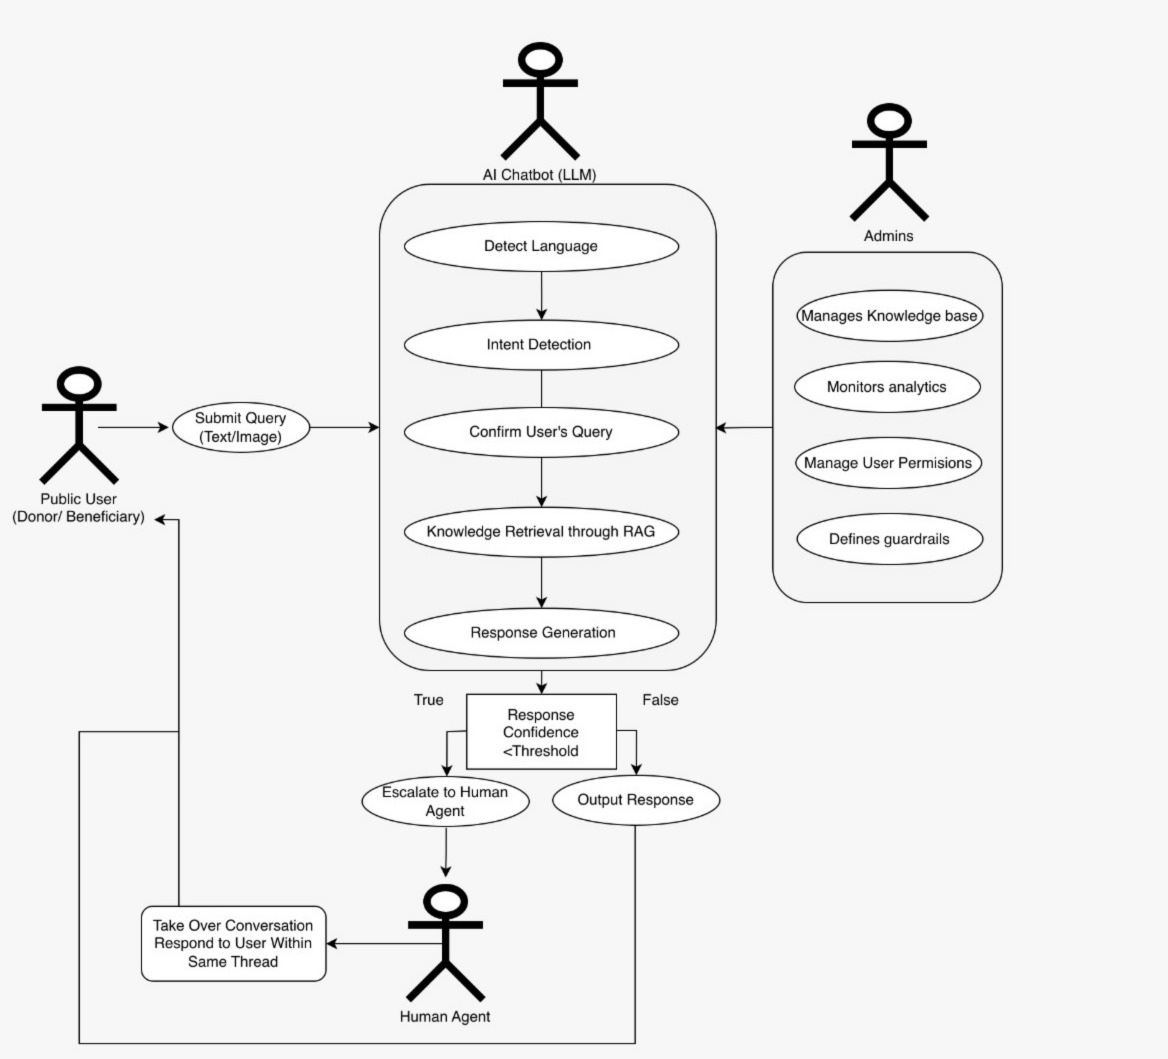
\includegraphics[width=0.9\textwidth]{chapters/srs usecase diagram.jpg}
    \caption{Use Case Diagram of the Public Chat Portal for Alkhidmat}
    \label{fig:usecase}
\end{figure}


\section{Non-functional Requirements}
\renewcommand{\arraystretch}{1.3}
\begin{longtable}{|p{3cm}|p{6.5cm}|p{6.5cm}|}
\caption{Non-Functional Requirements} \\
\hline
\textbf{Category} & \textbf{Description} & \textbf{Example} \\
\hline
\endfirsthead

\multicolumn{3}{c}%
{{\bfseries Table \thetable\ (continued): Non-Functional Requirements}} \\
\hline
\textbf{Category} & \textbf{Description} & \textbf{Example} \\
\hline
\endhead

\hline \multicolumn{3}{r}{{Continued on next page}} \\
\endfoot

\hline
\endlastfoot

\textbf{Performance} &
The system should respond within 3 to 15 seconds per query, depending on the complexity. &
Simple queries (e.g., blood bank locations) should return results in 3 seconds. Complex queries (e.g., eligibility criteria) may take up to 15 seconds. \\
\hline

\textbf{Accuracy and Relevance} &
Ensure the system provides $\geq$ 90\% accuracy and relevance in its responses to ensure reliability. &
If a user asks for blood donation instructions, the response should be factually correct and relevant in 90\% of cases. \\
\hline

\textbf{Usability / Accessibility} &
Support multilingual responses with consistent quality in both languages (e.g., English and Urdu). Include clear button-based flows for non-technical users. &
The system should provide responses in Urdu with the same clarity and accuracy as in English, without discrepancies. \\
\hline

\textbf{Reliability} &
Ensure the system maintains $>$ 90\% answer accuracy and minimal human routing. If accuracy falls below a threshold, route to a human agent. &
If a user asks for donation details and the system's confidence is below 70\%, it should route to a human agent. \\
\hline

\textbf{User Satisfaction (KPI)} &
Measure user satisfaction by asking for feedback 15--20 minutes after the last query with thumbs up/down ratings. &
After a session, if the user does not respond or replies with “no,” send a rating question (thumbs up/down) to evaluate the system's effectiveness. \\
\hline

\textbf{Data Integrity \& Backup} &
Ensure data accuracy and periodic backups of important data (e.g., RAG knowledge base). Implement automated weekly backups and data validation. &
Perform weekly automated backups of key data and ensure that data validation occurs during data entry to prevent corruption. \\
\hline

\textbf{Security / Compliance} &
Implement end-to-end encryption for all communications. Ensure no personal data retention beyond session lifetime. &
Personal data should not be retained after the session ends. The system should use encrypted communication protocols to secure sensitive information. \\
\hline

\textbf{Scalability} &
Support $\geq$ 500 simultaneous users without performance degradation using FastAPI + Elasticsearch on Docker/Heroku. &
The system should scale to support 500 simultaneous users accessing the platform without any degradation in response time. \\
\hline

\textbf{Maintainability} &
Use modular code architecture with clear documentation and API version control to ensure the system is easy to maintain and update. &
The codebase should be modular with proper documentation to allow for easy updates and troubleshooting. \\
\hline

\textbf{Compliance and Ethics} &
Adhere to Pakistan’s data privacy guidelines and AI ethics principles for NGO use. &
Ensure that the system follows local data privacy regulations and complies with ethical AI practices for non-profit organizations. \\
\hline

\end{longtable}

\section{System Diagram}
% This diagram gives a high-level view of the different components of our system and the interactions between them. Each component and the particular tools/technologies/libraries used to build it are described.
\begin{figure}[H]
    \centering
    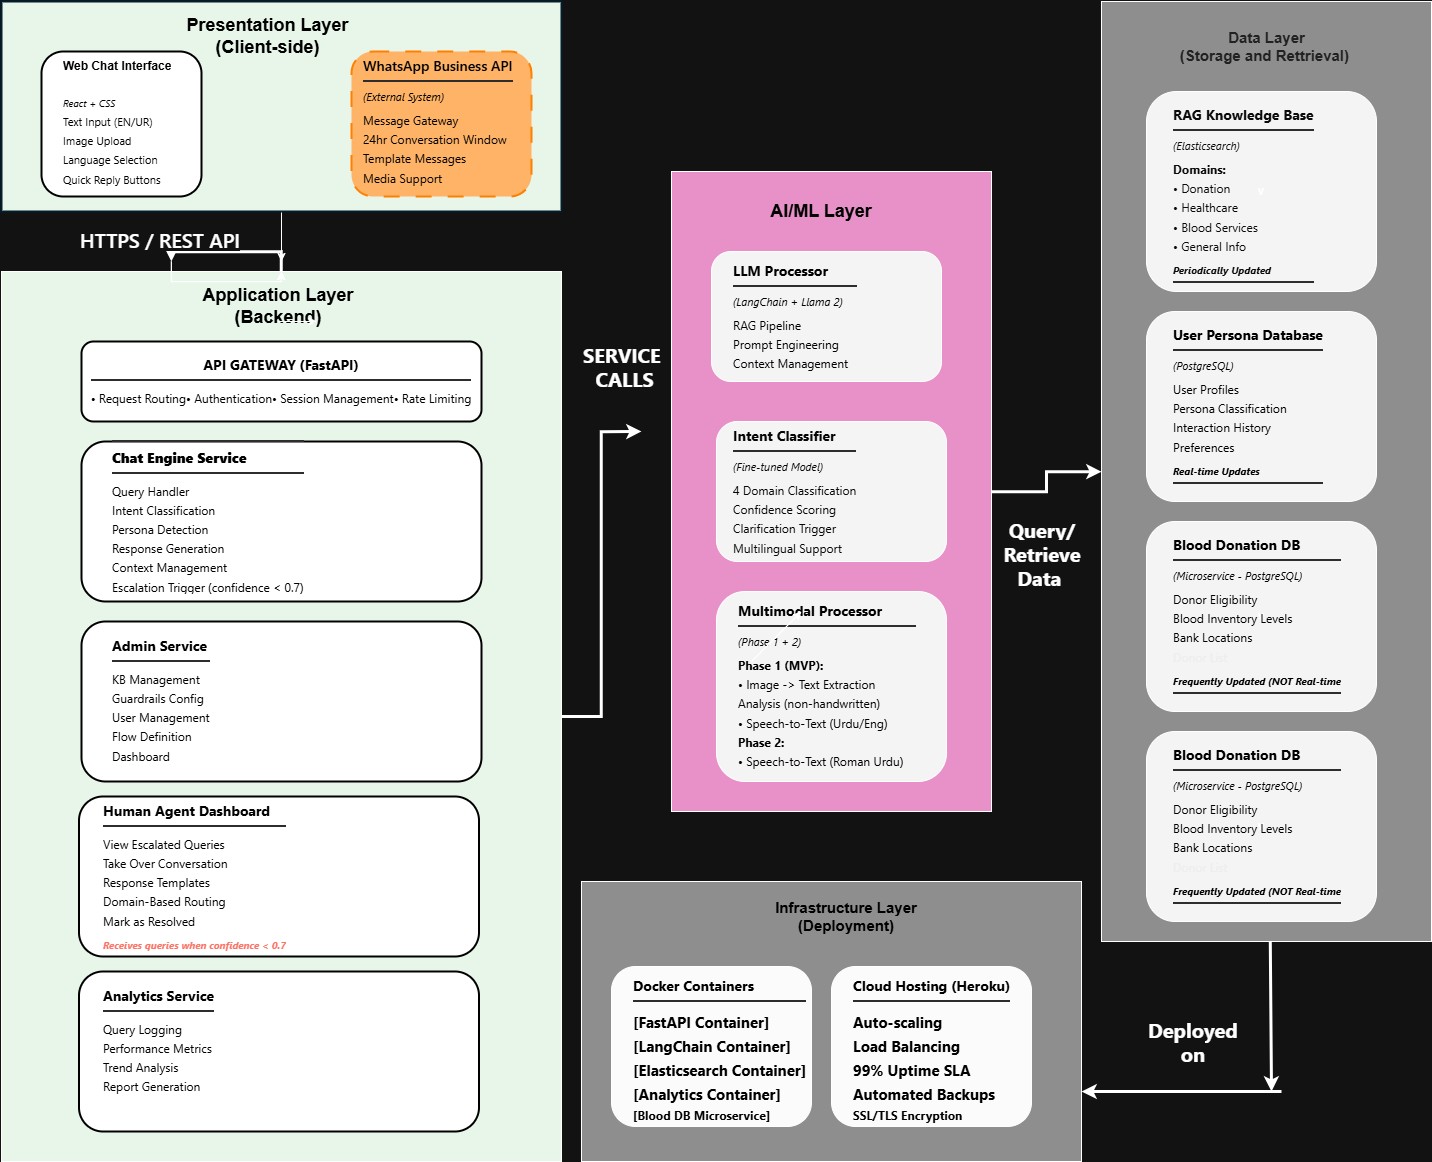
\includegraphics[width=1.1\textwidth]{chapters/high_level_architecture.drawio (1).png}
    \caption{High-level System Architecture}
    \label{fig:sysarchitecture}
\end{figure}
To view the diagram clearly, kindly access the following \href{https://app.diagrams.net/#G19okfbdDRLwywSZxlLuuXVhx5-wa4h22O#%7B%22pageId%22%3A%22drq8IgXnazhB2lmtOcQS%22%7D}{link.}
\\
The proposed system follows a five-layer architecture: Presentation Layer, Application Layer, AI/ML Layer, Data Layer, and Infrastructure Layer. Each layer plays a distinct role in ensuring efficient communication, scalability, and performance.

\subsection{Presentation Layer (Client-Side)}

\textbf{Components:}
\begin{itemize}
    \item \textbf{Web Chat Interface:} Built using React and CSS, enabling the user to interact with the system through a web interface. It supports features like text input (EN/UR), image uploads, language selection, and quick reply buttons.
    \item \textbf{WhatsApp Business API:} Used for external messaging functionalities such as managing conversations within a 24-hour window, sending template messages, and supporting media in chats.
\end{itemize}

\textbf{Role:} This layer is responsible for presenting the interface to the user, collecting user inputs, and initiating requests to the application layer via HTTP/REST APIs.

\subsection{Application Layer (Backend)}

\textbf{Components:}
\begin{itemize}
    \item \textbf{API Gateway:} Manages incoming requests, handles authentication, session management, and rate limiting.
    \item \textbf{Chat Engine Service:} Handles the main logic for query processing, intent classification, persona detection, and response generation. It also includes context management and escalation triggers for low-confidence queries.
    \item \textbf{Admin Service:} Provides tools for managing the knowledge base, user roles, and defining conversation flows.
    \item \textbf{Human Agent Dashboard:} Assists human agents in handling escalated queries, managing conversations, and routing them based on specific domains.
    \item \textbf{Analytics Service:} Logs queries, monitors performance metrics, and generates reports on system usage and trends.
\end{itemize}

\textbf{Role:} This layer is where the core processing happens. It handles requests from the presentation layer, processes them using the chat engine, and provides feedback to the user.

\subsection{AI/ML Layer}

\textbf{Components:}
\begin{itemize}
    \item \textbf{LLM Processor:} Processes the natural language input using large language models (LLMs) such as LangChain and Llama~2. It performs tasks like prompt engineering and context management.
    \item \textbf{Intent Classifier:} Classifies user inputs into predefined domains, scores confidence levels, and triggers escalation when confidence is low.
    \item \textbf{Multimodal Processor:} Handles input types like images or non-handwritten text and processes them into usable information, including support for Urdu and Roman Urdu.
\end{itemize}

\textbf{Role:} The AI/ML layer enhances the system's ability to process and understand user queries, making it capable of handling diverse input types and languages while maintaining context for more accurate responses.

\subsection{Data Layer (Storage and Retrieval)}

\textbf{Components:}
\begin{itemize}
    \item \textbf{RAG Knowledge Base:} Stores structured data related to donation, healthcare, and general services. This database is periodically updated.
    \item \textbf{User Persona Database:} Tracks user profiles, including interaction history, preferences, and persona classification, to provide personalized responses.
    % \item \textbf{Blood Donation Database:} Contains critical data on donor eligibility, blood inventory levels, and bank locations. This database is frequently updated.
\end{itemize}

\textbf{Role:} The data layer ensures that the necessary information is available for the application layer to process and retrieve during interactions. It stores both real-time and frequently updated data for accurate responses.

\subsection{Infrastructure Layer (Deployment)}

\textbf{Components:}
\begin{itemize}
    \item \textbf{Docker Containers:} Each component, including the FastAPI service, LangChain, Elasticsearch, and analytics, is containerized to ensure consistent and scalable deployment.
    \item \textbf{Cloud Hosting (Heroku):} The system is hosted on Heroku with auto-scaling, load balancing, and high availability (99\% uptime SLA). SSL/TLS encryption ensures secure communication.
\end{itemize}

\textbf{Role:} The infrastructure layer ensures that the system is deployed efficiently, scalable, and resilient. It handles the deployment of services and ensures they are readily available to process requests.

\subsection{Relationships Between Layers}

\begin{itemize}
    \item User interaction starts at the \textbf{Presentation Layer}, where the user inputs queries.
    \item Requests are routed via HTTPS/REST APIs to the \textbf{Application Layer} for processing.
    \item The \textbf{Chat Engine Service} in the Application Layer utilizes the \textbf{AI/ML Layer} to classify intents and process natural language queries.
    \item \textbf{Data Retrieval} from the Data Layer occurs through queries made by application services, which fetch relevant data from the knowledge base and databases.
    \item The system is deployed on the \textbf{Infrastructure Layer}, ensuring scalability and security.
\end{itemize}

\subsection{Flow of Interaction}

\begin{enumerate}
    \item \textbf{User Interaction} $\rightarrow$ Presentation Layer $\rightarrow$ API Gateway
    \item \textbf{Request Routing} $\rightarrow$ Chat Engine Service $\rightarrow$ AI/ML Layer (Intent Classification \& Response Generation)
    \item \textbf{Data Retrieval} $\rightarrow$ Data Layer (RAG Knowledge Base, User Persona)
    \item \textbf{Response Sent} $\rightarrow$ Presentation Layer $\rightarrow$ User (via WhatsApp or Web Chat)
\end{enumerate}

This architecture ensures that each layer is responsible for a specific aspect of the system, from front-end interaction to backend processing, AI-based intent classification, and data management, all underpinned by scalable and secure infrastructure.


\section{External Interfaces}
\subsection{User Interfaces - Wireframes}
% This section includes our mockup screens and briefly explains them.
\begin{figure}[H]
    \centering
    \includegraphics[width=1\textwidth]{chapters/whatsapp_ui.png}
    % 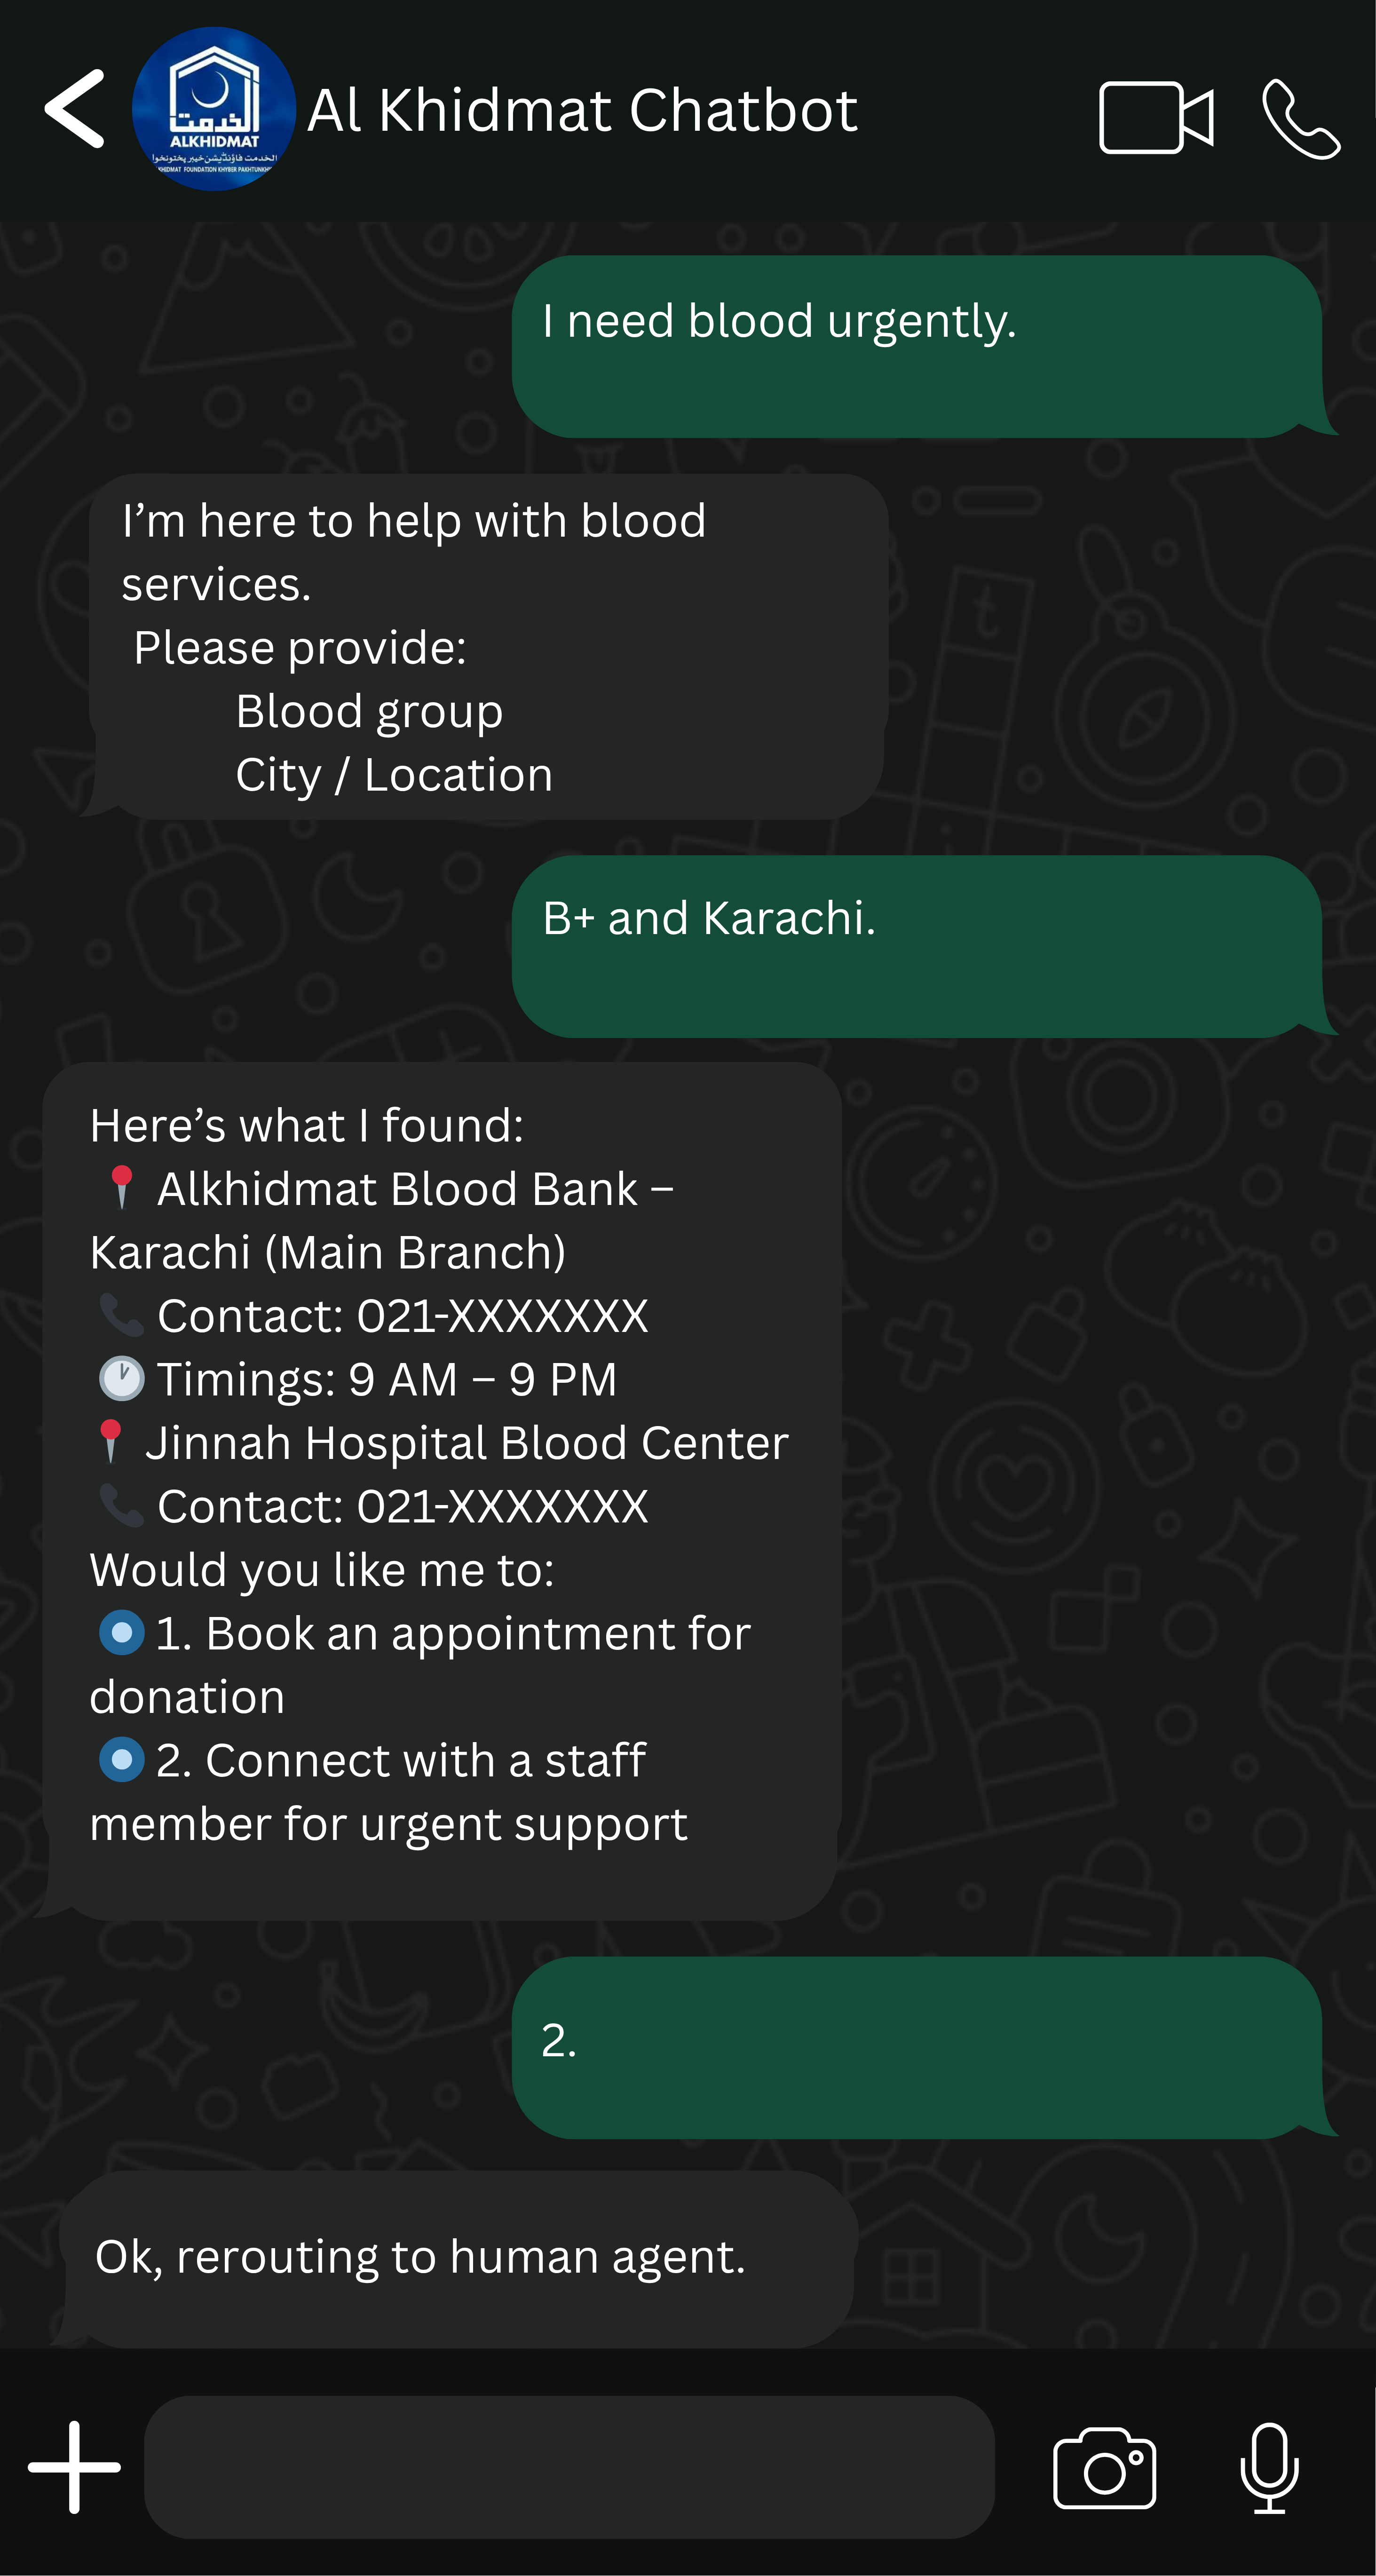
\includegraphics[width=0.335\textwidth]{chapters/chat2.png}
    \caption{User Interface using Whatsapp}
    \label{fig:UIuser}
\end{figure}

The two wireframes show how users might interact with the AI chatbot. Here, two use-cases are shown; monetary donors can select between Zakat, Sadaqah, or General Donations using quick buttons, receive verified payment options (Easypaisa, JazzCash, Visa/MasterCard), and obtain secure links with automated receipts, while complex or high-value cases are routed to human donation officers. Similarly, users seeking blood support can provide their blood group and city to instantly retrieve nearby Alkhidmat blood bank details and contact numbers; for urgent or unclear cases, the chatbot escalates the conversation to a live human agent within the same WhatsApp thread as we see in below wireframes. Both flows ensure verified information, user-friendly navigation, and human oversight for transparency and reliability.
\newpage
\begin{figure}[H]
    \centering
    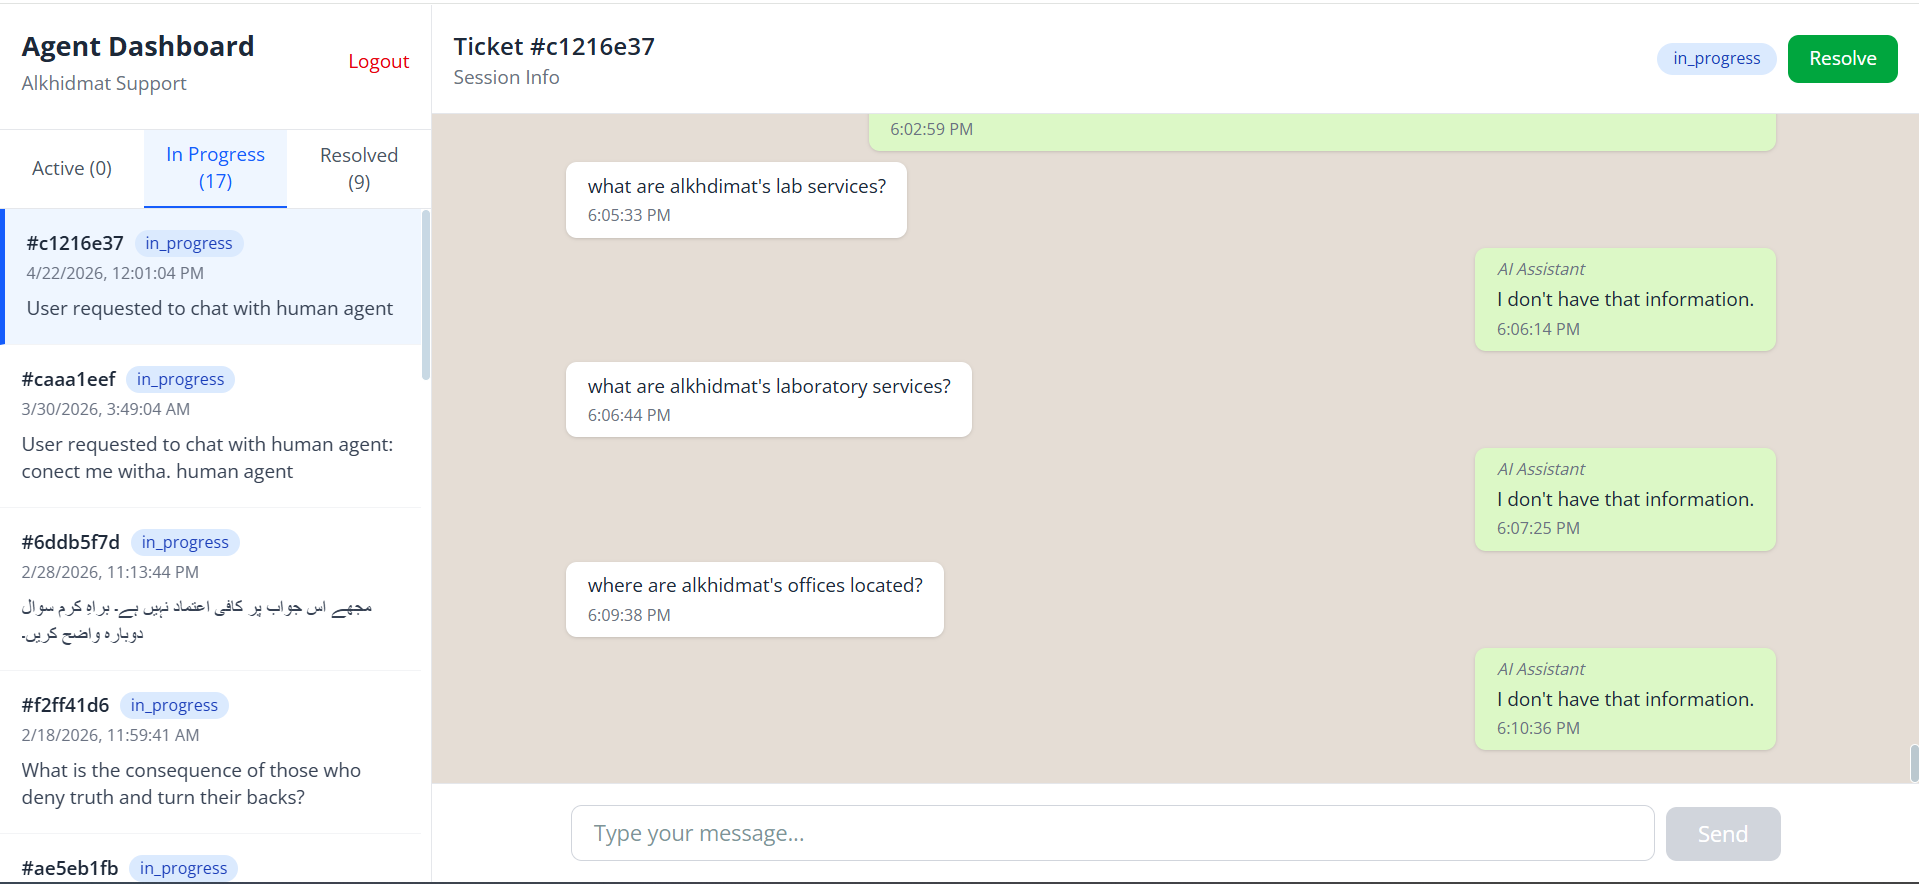
\includegraphics[width=1\textwidth]{chapters/Staff dashboard.png}
    \caption{Staff Dashboard}
    \label{fig:staffdashboard}
\end{figure}
If the AI bot is unable to confidently resolve any query, it will be escalated to Al-Khidmat's staff. The following is the dashboard where they will receive the queries.\\
The following example shows that the AI bit resolved a query with 8\% confidence, so it has been escalated to Fatima Ahmed, a human agent. She sees that there is a new ticket. She reviews the context where the user asked sensitive information and would personally guide her - all while updating the knowledge base for future training.
\\
The dashboard includes:
\begin{itemize}\setlength{\itemsep}{0pt}
    \item Left Panel: Live ticket queue with 4 realistic escalation scenarios (medical emergency, zakat calculation, scholarship, etc)
    \item Center Panel: Bilingual conversation thread showing bot-to-human handoff, where the agent has an option to transfer the query to another agent and resolve it once completed.
    \item Right Panel: User profile, escalation metadata, and knowledge base update form
\end{itemize}
\begin{figure}[H]
    \centering
    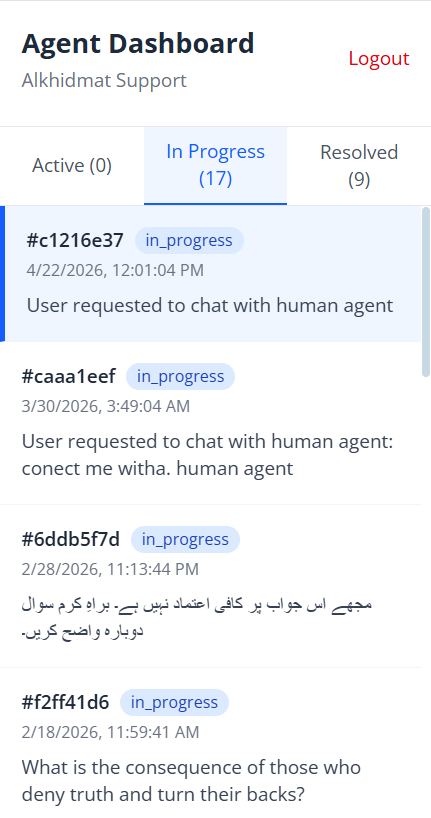
\includegraphics[width=0.5\textwidth]{chapters/ticket.png}
    \caption{Further Contents in Ticket Content Panel}
    \label{fig:ticketcontent1}
\end{figure}
% \begin{figure}[H]
%     \centering
%     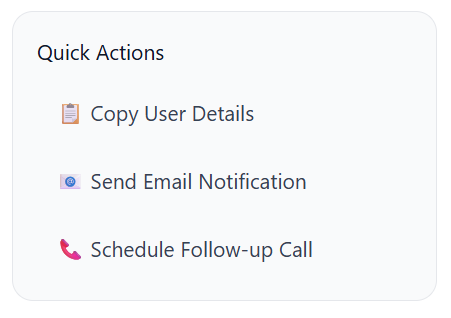
\includegraphics[width=0.5\textwidth]{chapters/Ticket Content 2.png}
%     \caption{Further Contents in Ticket Content Panel}
%     \label{fig:ticketcontent2}
% \end{figure}

\begin{figure}[H]
    \centering
    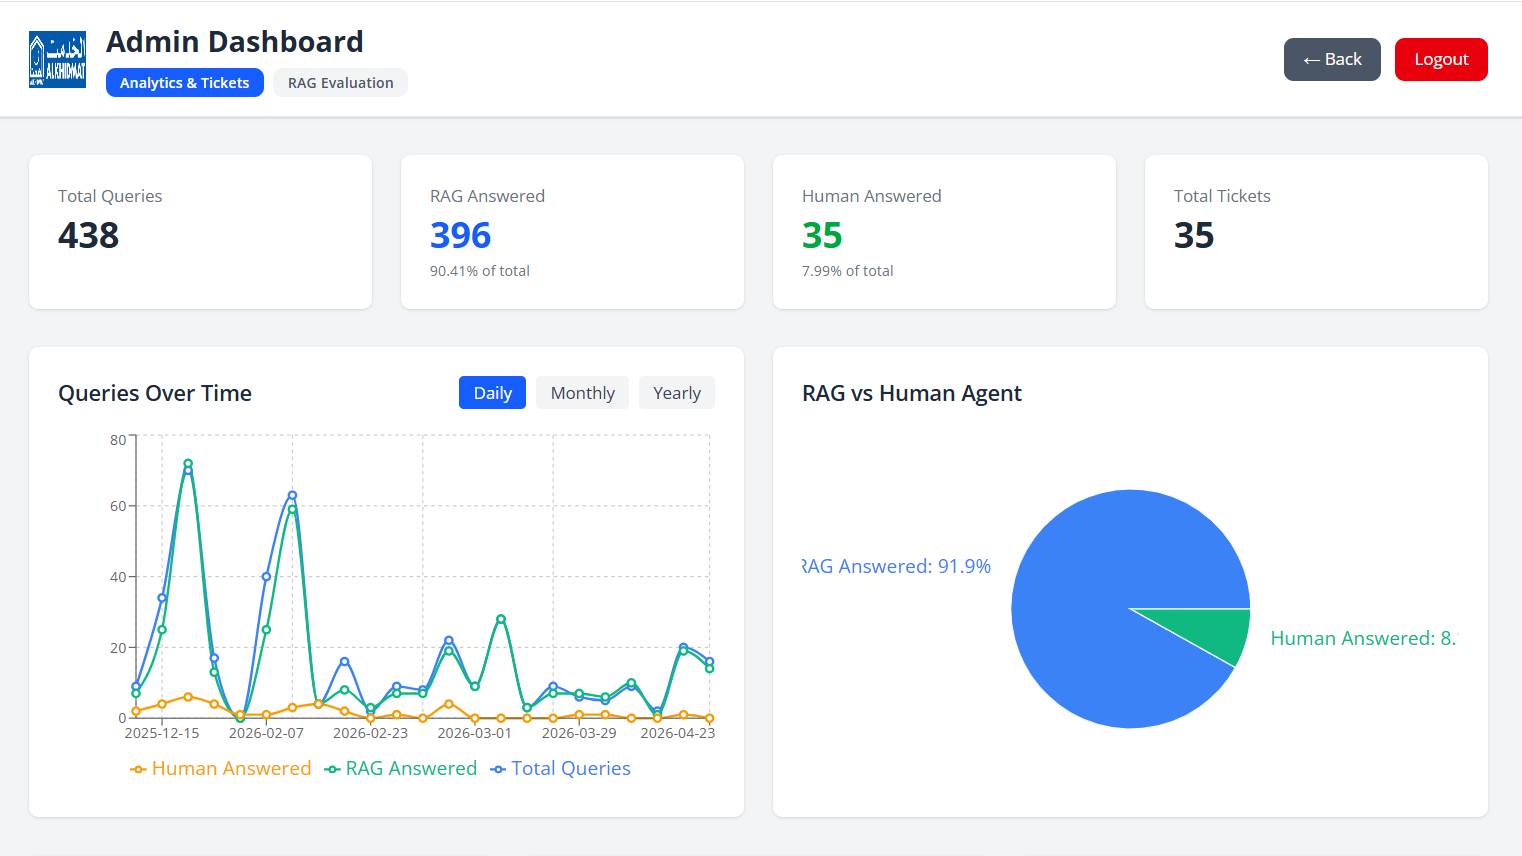
\includegraphics[width=0.9\textwidth]{chapters/dashboard.png}
    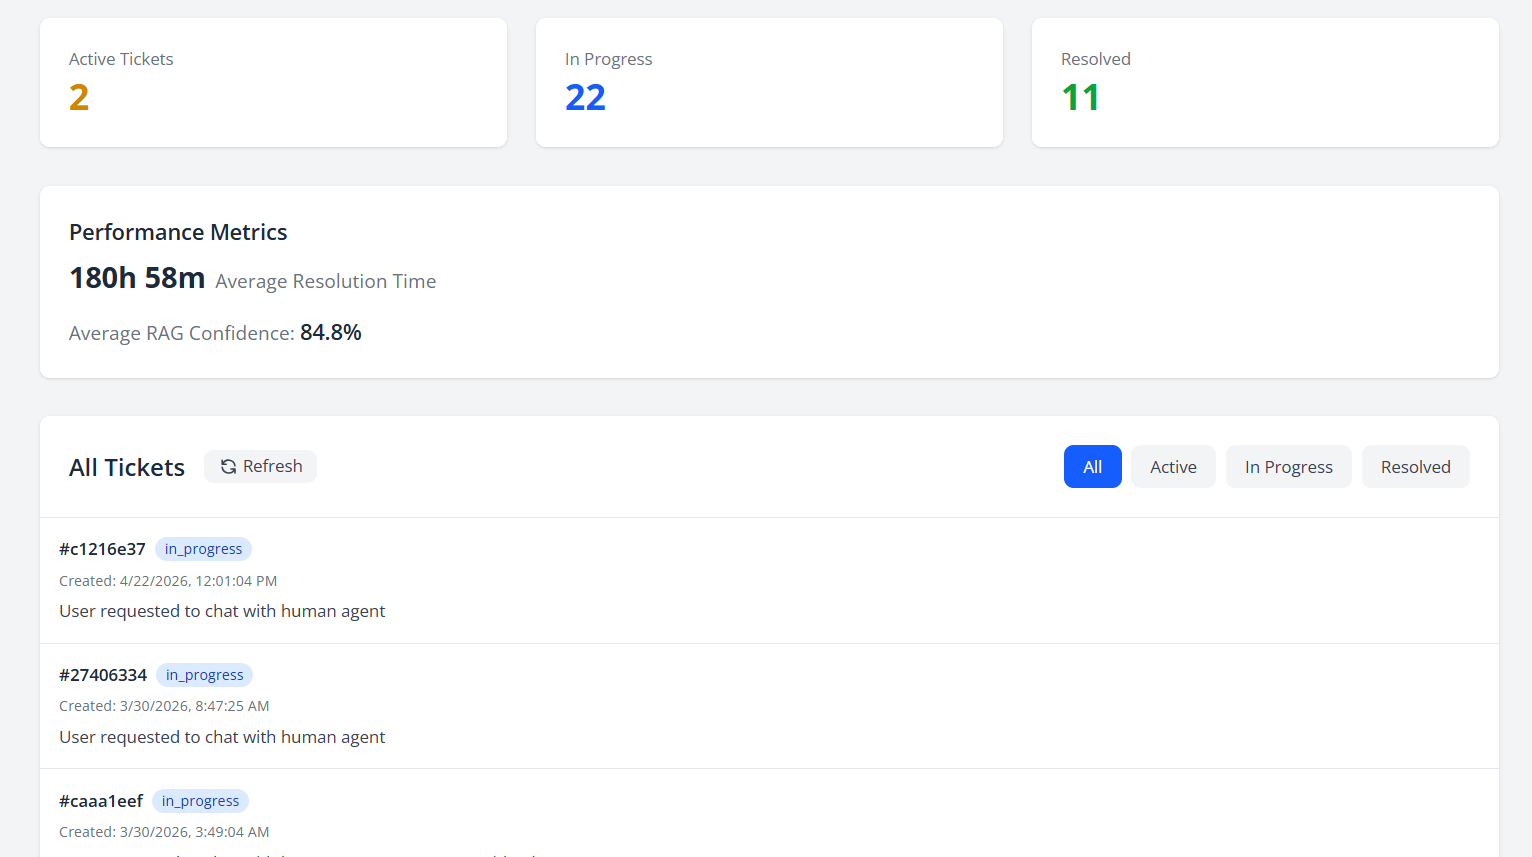
\includegraphics[width=0.9\textwidth]{chapters/dashboard_1.png}
    \caption{Admin's Dashboard - Analytics Monitor}
    \label{fig:analytics}
\end{figure}

The Analytics Dashboard features real-time tracking of chatbot performance and user activity, including domain-wise query distribution, daily and hourly interaction trends, and key usage metrics like total queries, average session time, and peak hours. It provides detailed insights into escalation rates, comparing AI-handled and human-assisted queries across domains to assess accuracy and efficiency. Additional features include a date selector for reviewing past analytics, visual charts for quick interpretation, and an intuitive, admin-friendly interface aligned with Alkhidmat Foundation’s branding for easy monitoring and performance optimization.

\begin{figure}[H]
    \centering
    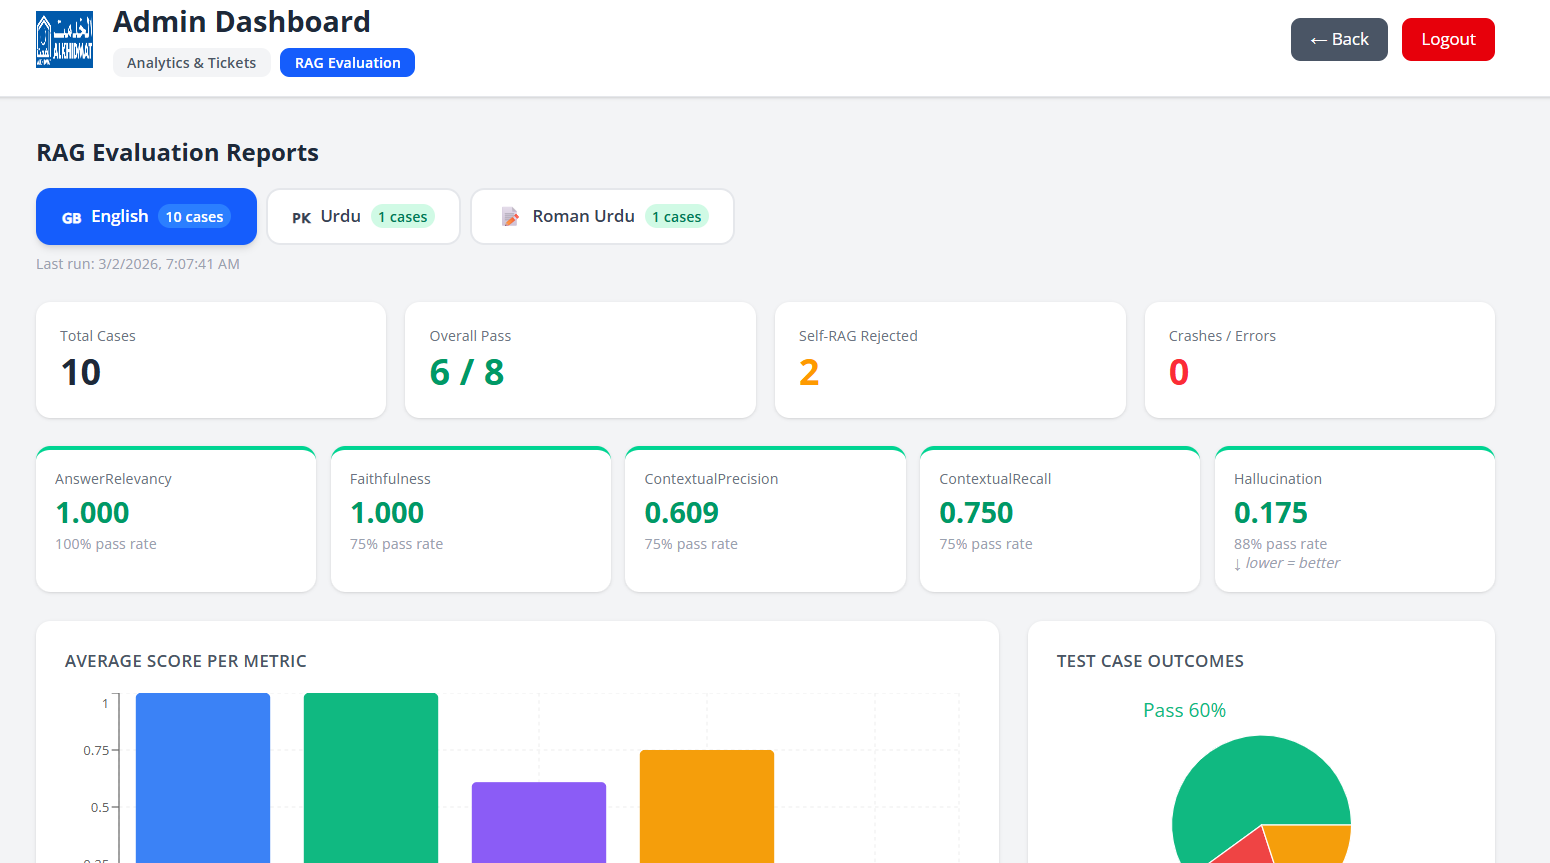
\includegraphics[width=0.9\textwidth]{chapters/RAG_eval.png}
    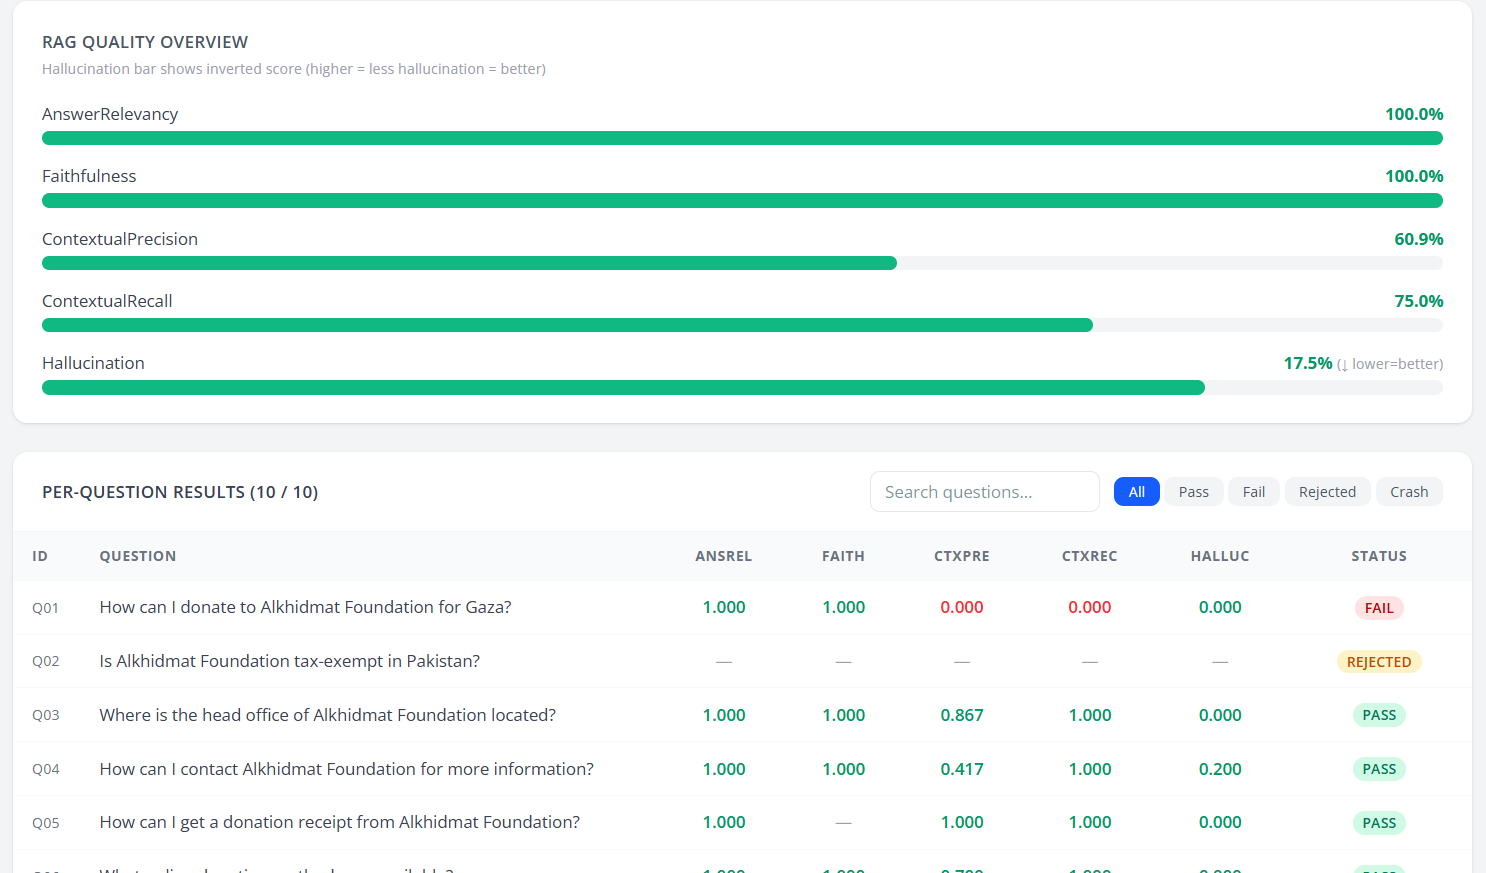
\includegraphics[width=0.9\textwidth]{chapters/RAG_eval_1.png}  
    \caption{Admin's Dashboard - RAG Evaluation}
    \label{fig:analytics_1}
\end{figure}
% \section{External Interfaces}

% We expect every project to have at least of the following subsections. This section must be aligned with your project deliverables. Please consult with your project supervisor regarding which of the following section(s) you should include in your report

% \subsection{Application Program Interface (API)}
% This section describes the library or API interface to our system.

% \subsection{Hardware/Communication Interfaces}
% This section describes our project's specific hardware/network interfaces.

% \section{Datasets}
% This section describes the specific dataset(s) used to build our system. An appropriate snapshot of the dataset(s) is also included. Futher details, when needed, are presented in the appendix.

